\section{Anforderungsanalyse}

\subsection{Stakeholder}
Im Rahmen der Bibliotheksanwendung lassen sich folgende Stakeholder identifizieren:
\\\textbf{Mitglieder} -- Nutzer der Bibliothek, die Bücher ausleihen, zurückgeben und ihren Kontostatus einsehen möchten.
\\\textbf{Mitarbeiterinnen und Mitarbeiter} -- Bibliothekspersonal, das Ausleihen und Rückgaben durchführt, Mitglieder verwaltet und bei Bedarf sperren oder freigeben kann.
\\\textbf{Administratorinnen und Administratoren} -- Mitarbeitende mit erweiterten Rechten, die Statistiken einsehen, Bücher verwalten und Auswertungen durchführen können.

\subsection{Personas}
\begin{figure}[H]
\vspace{-10pt}
  \centering
   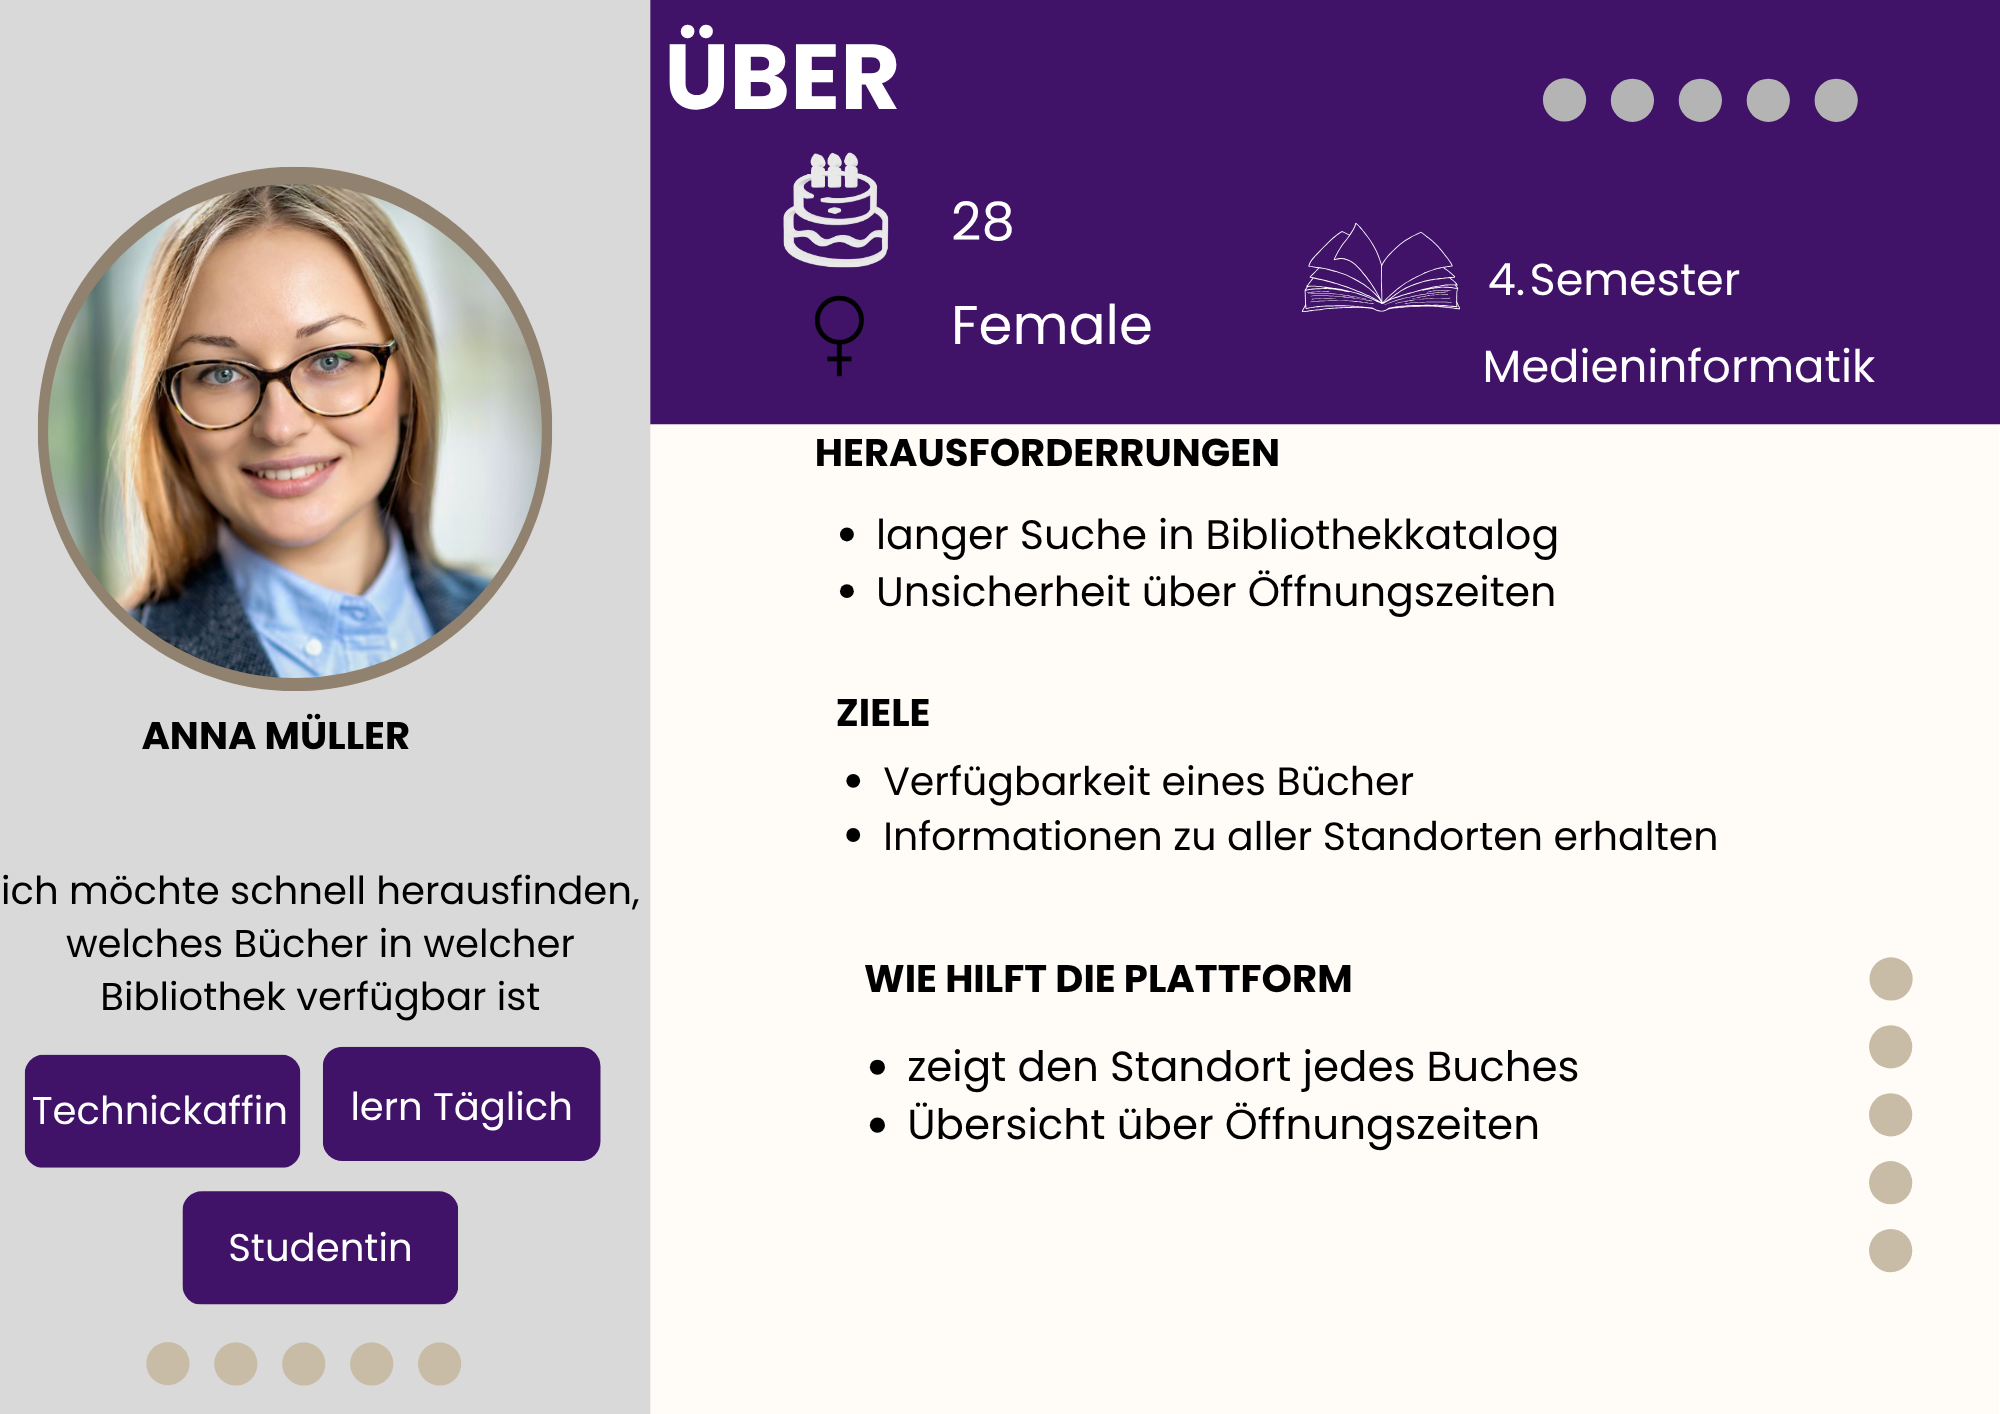
\includegraphics[width=0.9\linewidth]{src/abbildungen/persona1.png}
    \caption{Persona 1}
\vspace{-15pt}
\end{figure}
\begin{figure}[H]
  \centering
   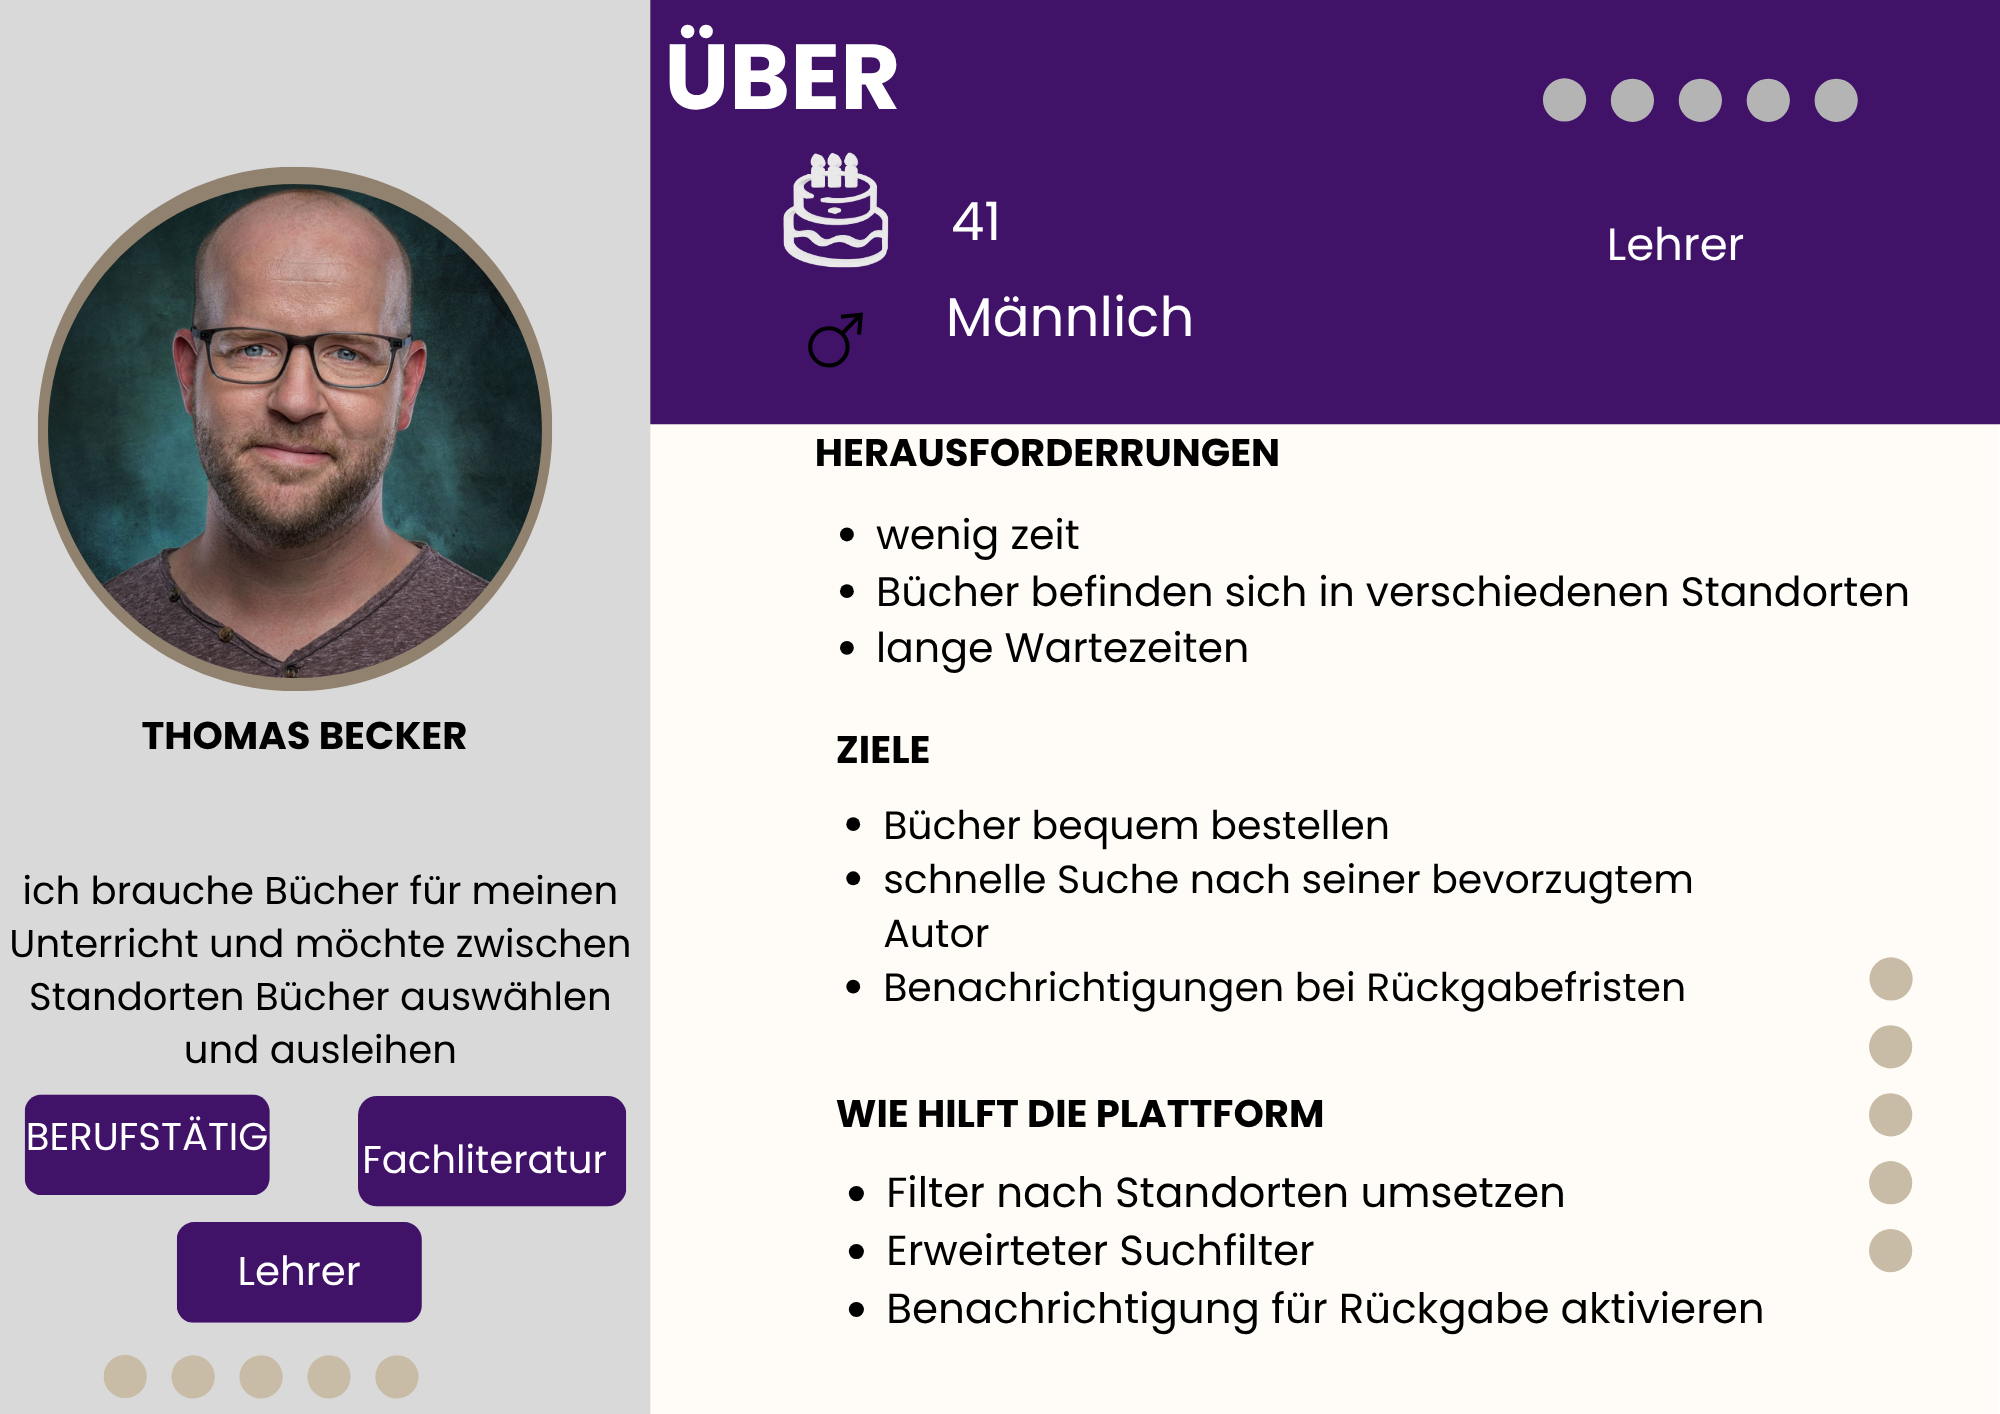
\includegraphics[width=0.9\linewidth]{src/abbildungen/persona2.png}
    \caption{Persona 2}
\vspace{-15pt}
\end{figure}

\subsection{Anforderungsanalyse}
\subsubsection{Funktionale Anforderungen}

\textbf{Mitglieder:}
Mitglieder können sich registrieren und einloggen. Auch ohne Anmeldung ist es möglich,
Bücher zu suchen und deren Verfügbarkeit nach Standort und Regal einzusehen.
Nach dem Login haben Mitglieder Zugriff auf ihre aktiven Ausleihen mit Fälligkeitsdatum
und anfallenden Mahngebühren sowie auf ihre Ausleihhistorie.
Gesperrte Mitglieder erhalten eine Anzeige mit dem jeweiligen Sperrgrund.

\textbf{Mitarbeiterinnen und Mitarbeiter:}
Mitarbeitende authentifizieren sich mit E-Mail, Passwort und Mitarbeiter-ID.
Sie erfassen Ausleihen, indem sie die Ausweisnummer des Mitglieds und mehrere
Barcodes nacheinander einscannen und die Ausleihe anschließend bestätigen.
Bei der Rückgabe können mehrere Bücher gleichzeitig bearbeitet werden,
wobei der Zustand jedes Buches erfasst wird. Mahngebühren werden automatisch
mit 0{,}10~Euro pro Tag nach Ablauf der Leihfrist berechnet.
Darüber hinaus können Mitarbeitende Mitglieder suchen, ihre Ausleihhistorie einsehen
sowie Mitglieder manuell mit Angabe eines Grundes sperren oder freigeben.

\textbf{Administratorinnen und Administratoren:}
Admins haben Zugriff auf eine Übersicht mit Kennzahlen wie Bestand, aktive Ausleihen,
überfällige Ausleihen und gesperrte Mitglieder. Sie können Bücher suchen,
hinzufügen -- mit Angabe von Autor, Standort, Regalnummer und Exemplaranzahl --
sowie aus dem Bestand entfernen. Zusätzlich stehen Autorenstatistiken,
gefilterte Mitgliederübersichten und Auswertungen nach Zeitraum zur Verfügung.

\subsubsection{Nicht-funktionale Anforderungen}

\textbf{Sicherheit:}
Authentifizierung erfolgt sitzungsbasiert; Session Fixation wird verhindert.
Der Zugriff auf geschützte Seiten wird serverseitig durch einen Servlet-Filter (\texttt{MyFilter}) geregelt.
Nicht autorisierte Zugriffsversuche werden auf die Login-Seite umgeleitet.

\begin{figure}[H]
\vspace{-10pt}
  \centering
   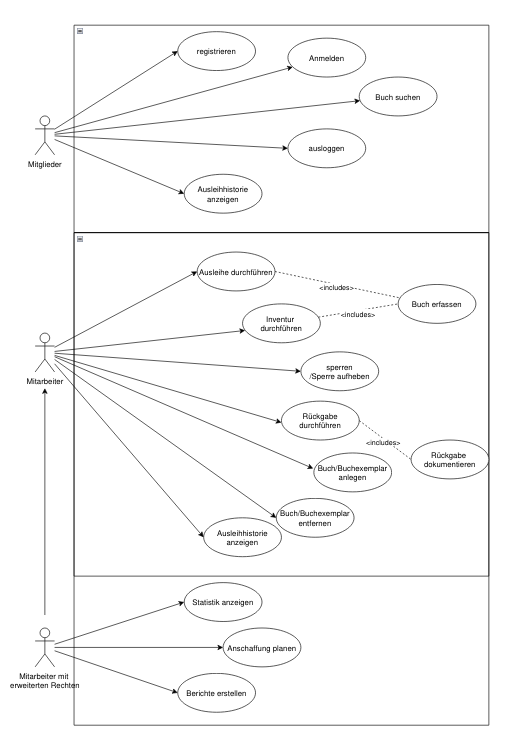
\includegraphics[width=0.9\linewidth]{src/abbildungen/usecase_swe2.png}
    \caption{Use Case}
\vspace{-15pt}
\end{figure}
